\section{How strongly does incident heating change the answer?}\label{sec:film}
The following exposures start at 22 $^\circ$C, with bare phenolic facing 2504 K gas
at 800 psi. Each column changes the gas-side film coefficient before blowing,
$h_0$, in W/(m$^2$ K). Wall temperature, gas release, char consumption and
the casing response evolve together. The first three columns give the time
to consume the original liner, including its char. The last three show when
all aluminium cells become liquid or the hottest CF casing cell reaches
1000 $^\circ$C. Times are in seconds.
\begin{table}[H]\centering\begin{tabular}{lrrr@{\hspace{1.6em}}rrr}\toprule
 & \multicolumn{3}{c}{Liner exhausted} & \multicolumn{3}{c}{Casing event}\\
$h_0$ & 500 & 1000 & 2000 & 500 & 1000 & 2000 \\\midrule
Sustainer Al & 206.9 & 110.5 & 60.2 & 170.7 & 99.1 & 56.9 \\
Sustainer CF & 195.4 & 104.3 & 56.6 & --- & 95.1 & 51.3 \\
Booster Al & 276.4 & 147.6 & 80.4 & 248.8 & 139.4 & 77.8 \\
Booster CF & 258.7 & 137.9 & 74.8 & --- & 129.7 & 69.7 \\
\bottomrule\end{tabular}\end{table}
The dash means the CF surrogate stayed below 1000 $^\circ$C until exhaustion.
All four casings exceeded their original material-property flags at all three
loads. The calculation retains the molten metal or decomposed composite in place.
\begin{figure}[H]\centering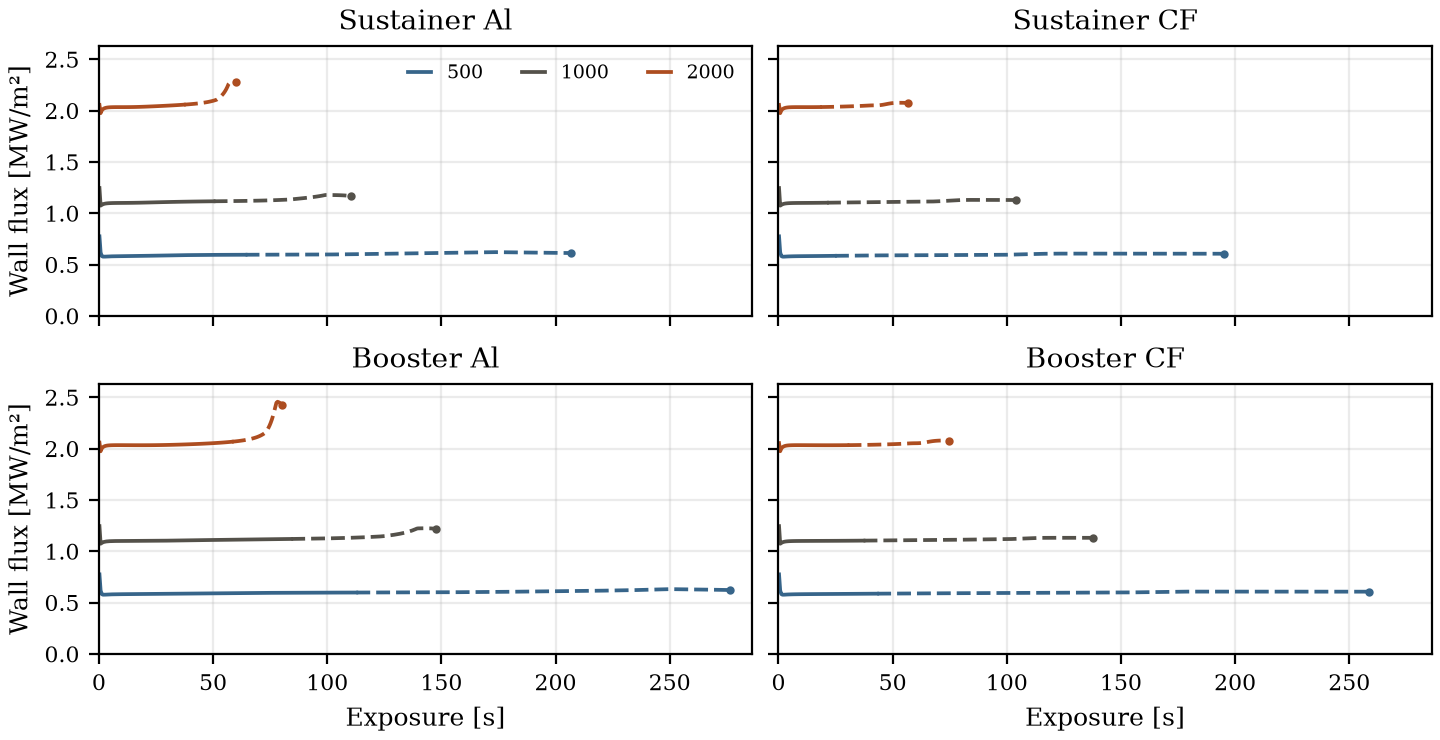
\includegraphics[width=0.98\textwidth]{../analysis/evolving_backing_heat_flux.png}
\caption{Modelled convective heat entering the receding surface over each
half-second interval and the final partial interval. Colours identify $h_0$.
Dashes start at the first 300 $^\circ$C Al or 150 $^\circ$C CF interface flag.
The final dot marks the mean over the last interval before liner loss.}
\end{figure}
The film changes the rate at which energy enters the wall. Even with a fixed
gas temperature and $h_0$, the driving temperature difference falls as the
surface heats, and gas from the liner suppresses convection. The actual
incident load requires a firing measurement or an independently validated
gas-side calculation.
\clearpage
\section{Heat delivered to the receding surface and numerical checks}
For one radian of circumference and one metre of axial length, the exposed
area equals its instantaneous radius $r_s$ in SI units. Each saved interval
provides its convective energy $\Delta E_f$, including the blowing correction.
The plotted flux divides this energy by the duration and average endpoint area.
Because the surface moves monotonically outwards, the two endpoint areas
also enclose the exact area--time integral. For the full exposure,
\[
 \frac{\sum\Delta E_f}{\sum r_{j+1}\Delta t_j}
 \leq \overline{q''}_f =
 \frac{\int q''_f r_s\,dt}{\int r_s\,dt}
 \leq \frac{\sum\Delta E_f}{\sum r_j\Delta t_j}.
\]
The table gives the midpoint of these bounds in MW/m$^2$. Across all
twelve histories their largest half-width is 1.022 kW/m$^2$. The last column
gives cumulative film energy per original exposed area across the three loads.
\begin{table}[H]\centering\begin{tabular}{lrrrr}\toprule
 & \multicolumn{3}{c}{Mean flux [MW/m$^2$]} & Energy per original area\\
$h_0$ [W/(m$^2$ K)] & 500 & 1000 & 2000 & [MJ/m$^2$] \\\midrule
Sustainer Al & 0.603 & 1.126 & 2.074 & 131.9--132.6 \\
Sustainer CF & 0.598 & 1.114 & 2.045 & 122.5--123.4 \\
Booster Al & 0.603 & 1.128 & 2.079 & 174.8--175.6 \\
Booster CF & 0.597 & 1.113 & 2.043 & 160.2--161.6 \\
\bottomrule\end{tabular}\end{table}
\paragraph{Checking each heating level.}
For each of the eight new combinations, the finite-volume calculation was
repeated with 320/80 and 640/160 liner/casing cells at a 0.04 s step ceiling,
then with 640/160 cells at 0.02 s. An accepted pair must have overlapping
event brackets, less than 5\% endpoint change and matched thickness within
the larger of 0.02 mm and 1\% of original thickness. Booster Al at 2000 required additional time refinement. At 640/160 cells, the last two step ceilings were 0.005 and 0.0025 s. Their endpoints differed by 0.0013 s.

A second radial finite-element calculation used 160/40 cells and a 0.02 s
ceiling from ignition in all eight cases. Across those cases the two methods
differ by at most 0.127 s at exhaustion, 0.0066 mm of liner on
common reporting times, and 10.93 K at the casing interface. For the
finite-volume records the largest fractional mass imbalance is $2.2\times 10^{-12}$ and
the largest heat imbalance relative to incident energy is $9.8\times 10^{-12}$.
These checks quantify numerical agreement for the stated closures.
\paragraph{What still controls the physical answer.}
In this calculation gas impinges directly on bare phenolic until its last
material is removed. Actual ignition-to-exposure delay, burn duration, casing
retention and circumferential hot spots can change the result. A local
heat-flux history and pre/post-fire liner profiles at the same station would
test both the imposed load and the predicted loss. The table on the preceding
page gives a sensitivity to load, with no assigned probability.
\clearpage
